\section{支持向量机}
\label{sec:chapter10}

\subsection{优化目标}

逻辑回归的优化目标为：
\[
\min_\theta\frac{1}{m}\left[\sum_{i=1}^my^{(i)}\left(-\ln h_\theta(x^{(i)})\right)+(1-y^{(i)})\left(-\ln (1-h_\theta(x^{(i)}))\right)\right]+\frac{\lambda}{2m}\sum_{j=1}^n\theta_j^2
\]
将 $-\ln h_\theta(x^{(i)})$ 记为 $\text{cost}_1(\theta^T x^{(i)})$，它表示样本类别为 $1$ 时的代价；将 $-\ln(1-h_\theta(x^{(i)}))$ 记为 $\text{cost}_0(\theta^T x^{(i)})$，它表示类别为 $0$ 时的代价。支持向量机不再通过 sigmoid 函数得到平滑的对数代价，而使用如下分段线性函数近似：
\[
\text{cost}_1(z)=\begin{cases}0&z\geqslant1\\k_1(z-1)&z<1\end{cases}\quad\quad
\text{cost}_0(z)=\begin{cases}0&z\leqslant-1\\k_0(z+1)&z>-1\end{cases}
\]

\begin{figure}[H]
    \centering
    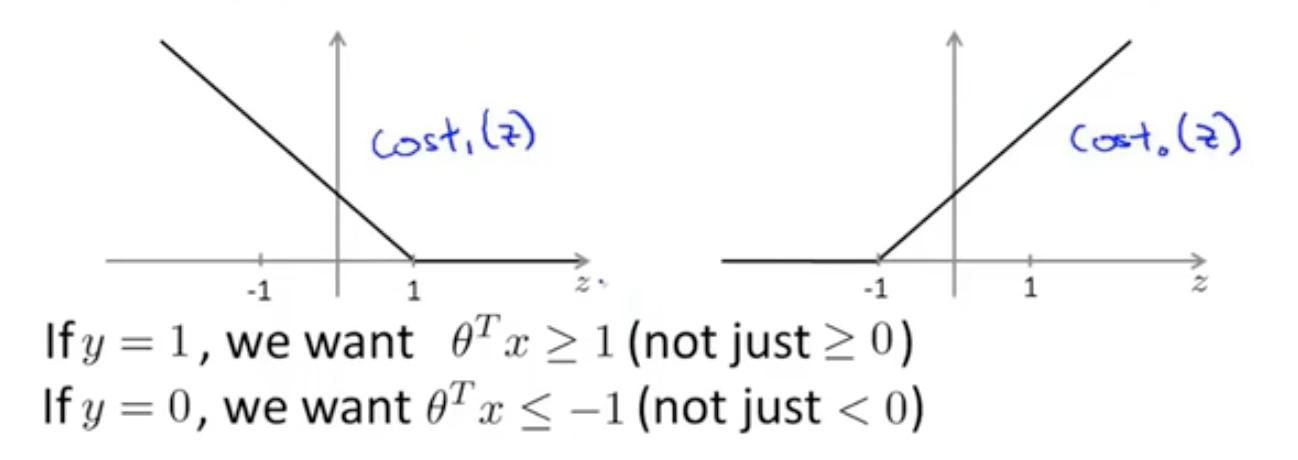
\includegraphics[width=0.6\linewidth]{figs/Chap_10_cost.png}
\end{figure}

在支持向量机的常用写法中，通常省略除以样本数 $m$ 的系数，并将正则化参数置于第一项而不是第二项。故支持向量机的优化目标为：
\[
\boxed
{\min_\theta C\sum_{i=1}^m\left[y^{(i)}\text{cost}_1(\theta^Tx^{(i)})+(1-y^{(i)})\text{cost}_0(\theta^Tx^{(i)})\right]+\frac{1}{2}\sum_{j=1}^n\theta_j^2}
\]
其中，$C$ 是正则化参数，用于权衡分类误差与参数规模，其作用与逻辑回归中的 $\frac{1}{\lambda}$ 类似：$C$ 越大，对训练样本分类错误的惩罚越强。

\begin{remark}
先考察 $y\text{cost}_1(\theta^Tx)+(1-y)\text{cost}_0(\theta^Tx)$ 这一分类代价。理想情况下，希望 $\text{cost}_y(\theta^T x)=0$，这对应 $\begin{cases}\theta^Tx\geqslant 1&\text{if }y=1\\\theta^Tx\leqslant -1&\text{if }y=0\end{cases}$. 以类别 $1$ 为例，逻辑回归只需要比较 $\theta^Tx$ 与 $0$ 的大小便可作出分类，而支持向量机还要求 $\theta^Tx$ 至少达到 $1$. 这意味着样本不仅要位于决策边界正确的一侧，还要与边界保持一定间隔。

从几何角度看，$\theta^Tx$ 是向量 $\theta$ 与 $x$ 的点积，可以理解为 $x$ 在 $\theta$ 方向上的投影与 $\theta$ 长度的乘积。$||\theta||$ 表示参数向量的长度，而正则化项 $\sum\limits_{j=1}^n\theta_j^2$ 等于 $||\theta||$ 的平方。减小参数长度相当于增大决策边界两侧的几何间隔，因此第二项体现了最大间隔的目标。$C$ 较大时，模型更重视让训练样本满足分类条件，即使这需要较大的参数；$C$ 较小时，模型允许少量样本被错误分类或落入间隔内部，以换取更大的分类间隔和更强的正则化。

\begin{figure}[H]
    \centering
    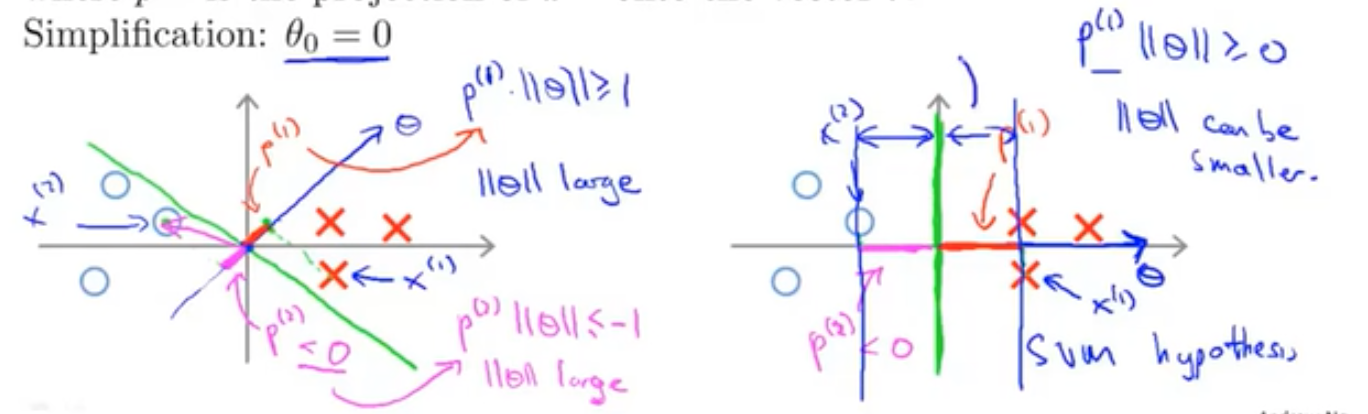
\includegraphics[width=\linewidth]{figs/Chap_10_big_margin.png}
\end{figure}

\end{remark}


\subsection{核函数}

对于在原特征空间中无法用直线或超平面分开的数据，可以引入核函数 $\phi:x\mapsto \phi(x)$，将原始 $n$ 维向量映射到更高维的特征空间。原空间中的非线性边界可能对应新空间中的线性边界，因此仍可使用线性支持向量机进行分类。常用核函数包括：

\textbf{线性核}：保持原特征不变
\[
\phi(x_i)=x_i
\]

\textbf{高斯核}
\[
\phi(x)=\begin{bmatrix}\exp\left(-||x-l^{(1)}||^2/2\sigma^2\right)\\\exp\left(-||x-l^{(2)}||^2/2\sigma^2\right)\\\vdots\\\exp\left(-||x-l^{(m)}||^2/2\sigma^2\right)\end{bmatrix}
\]
其中 $\sigma$ 控制相似度随距离衰减的速度，$l^{(1)},\cdots,l^{(m)}$ 称为 landmark. 每个新特征衡量输入 $x$ 与某个 landmark 的接近程度；实践中通常直接采用训练样本 $x^{(1)},\cdots,x^{(m)}$ 作为 landmark.


\subsection{代码实现}

\paragraph{线性可分情形}

首先观察数据集：

\begin{figure}[H]
    \centering
    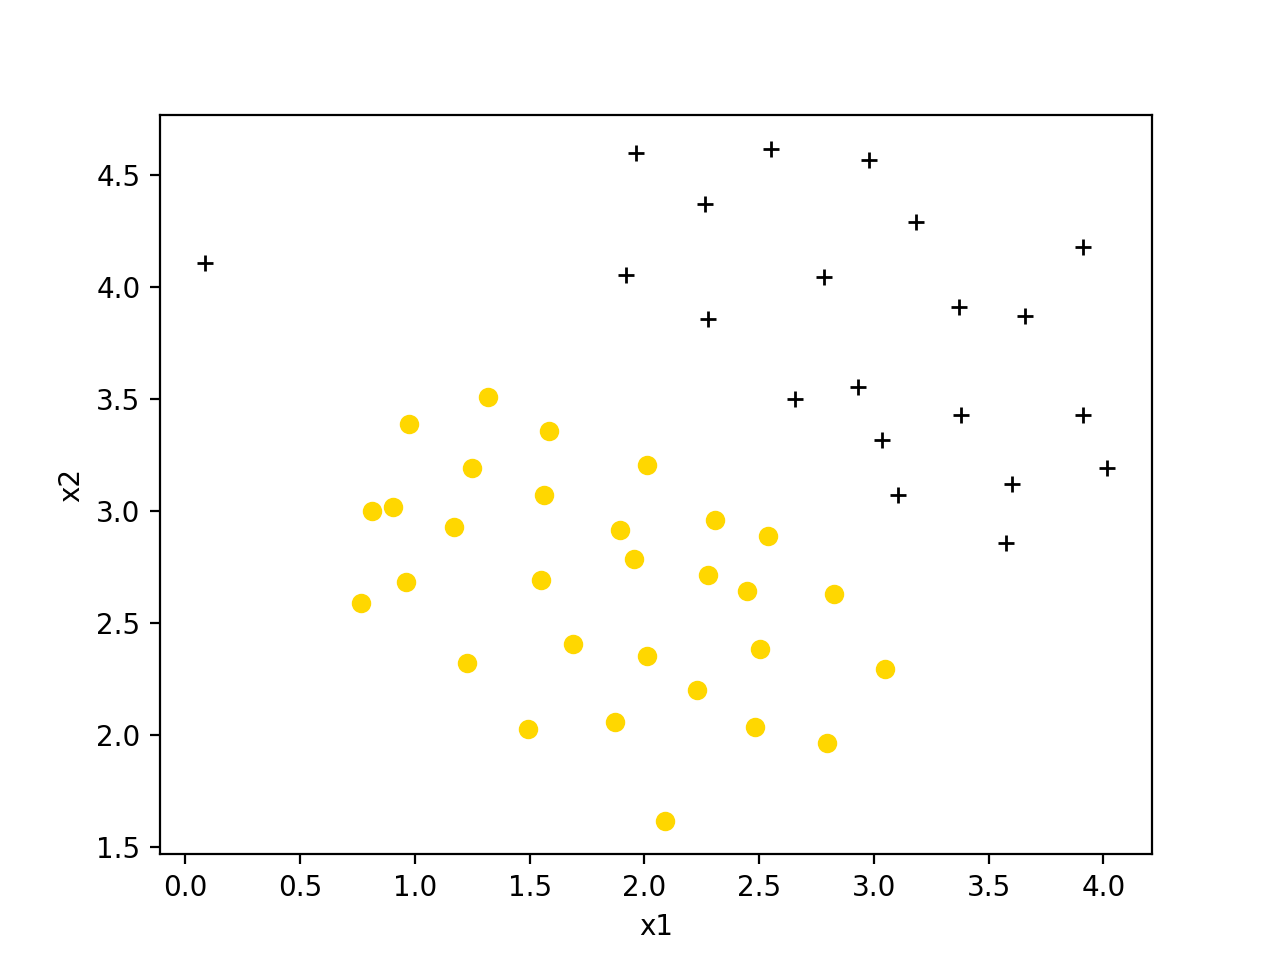
\includegraphics[width=0.4\linewidth]{figs/Chap_10_Figure_1.png}
\end{figure}

\begin{lstlisting}[language=Python]
from sklearn import svm

clf = svm.SVC(C=1, kernel='linear')
clf.fit(X, y)
\end{lstlisting}

训练结果如下：

\begin{figure}[H]
    \centering
    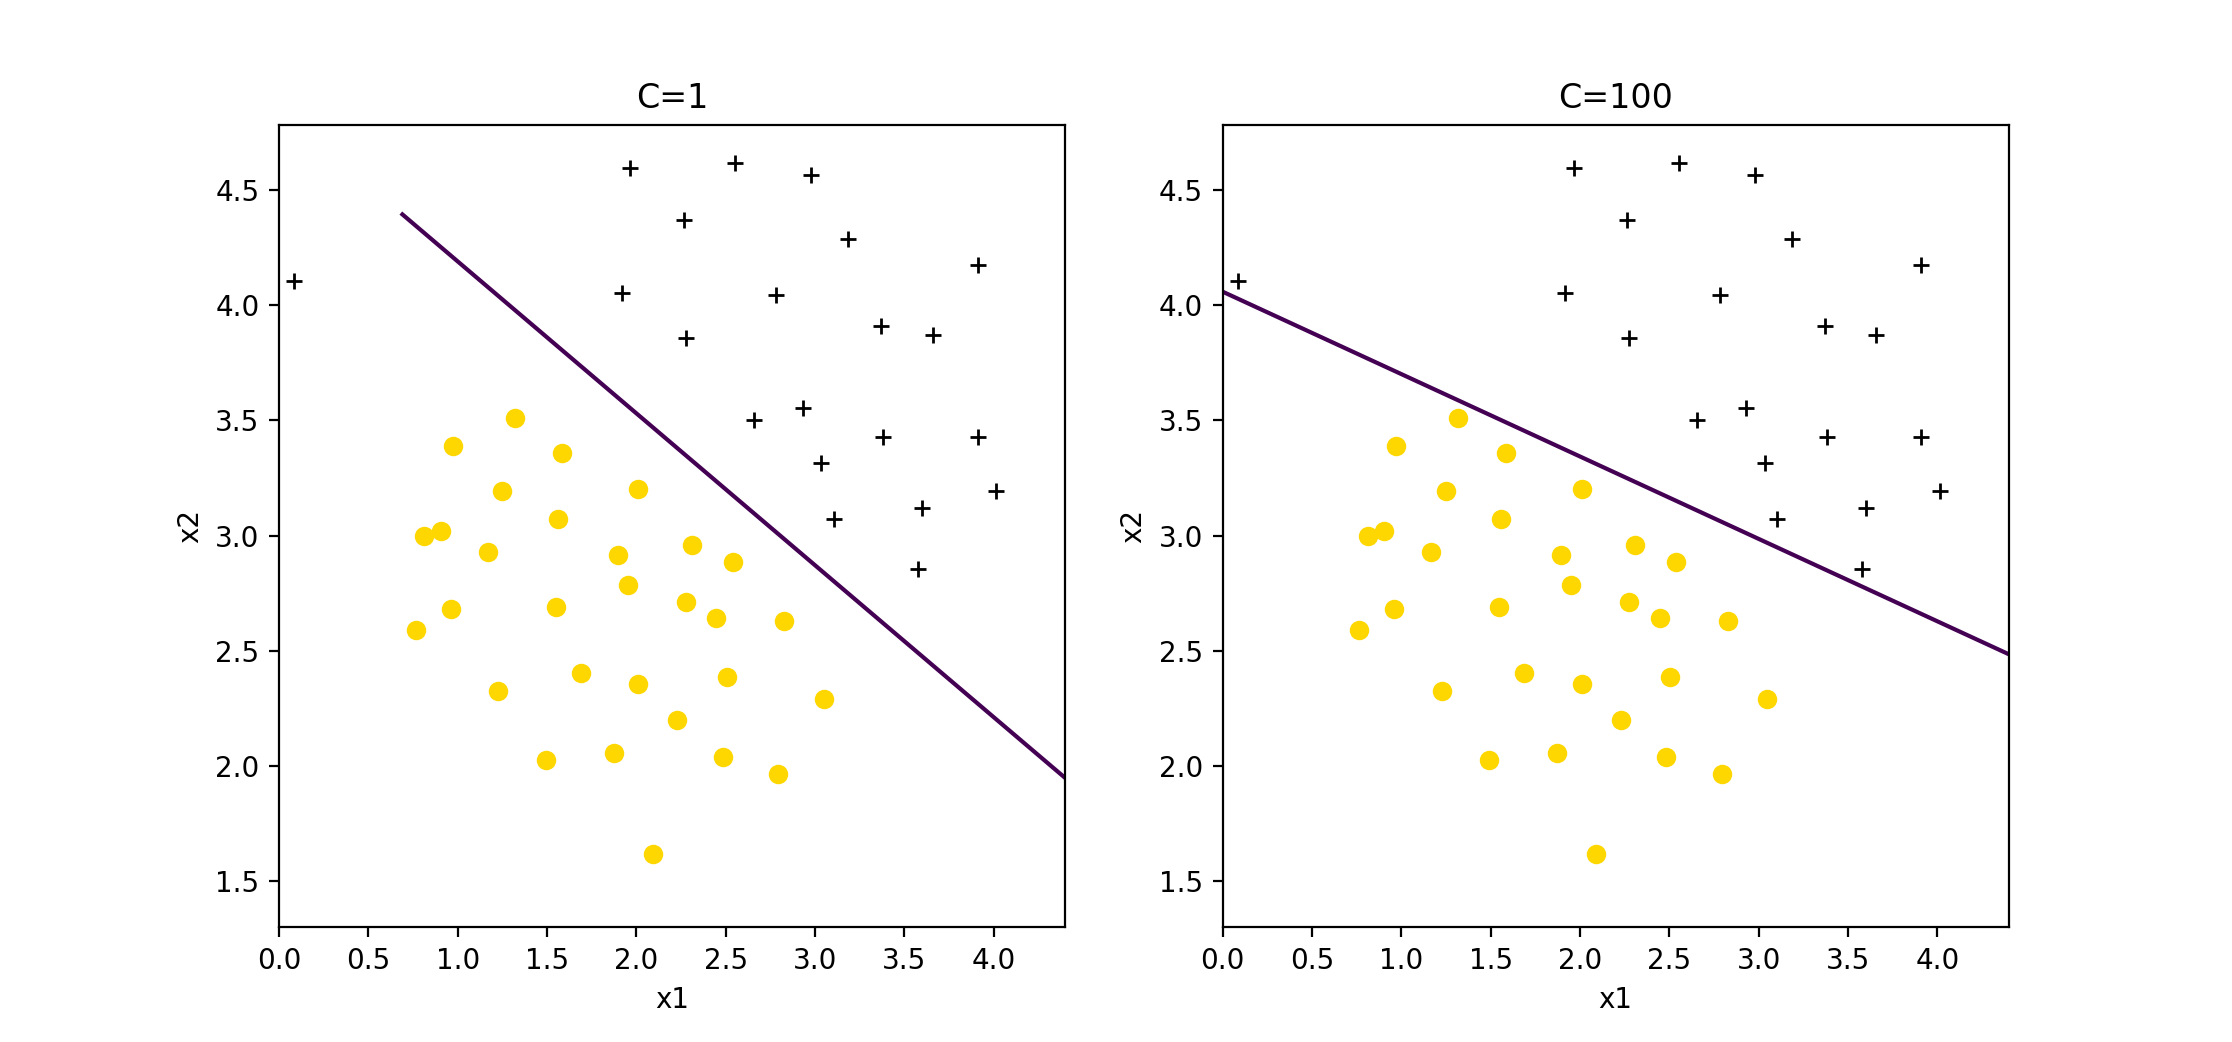
\includegraphics[width=0.8\linewidth]{figs/Chap_10_Figure_1_1.png}
\end{figure}


\paragraph{带高斯核的 SVM}

首先观察数据集：

\begin{figure}[H]
    \centering
    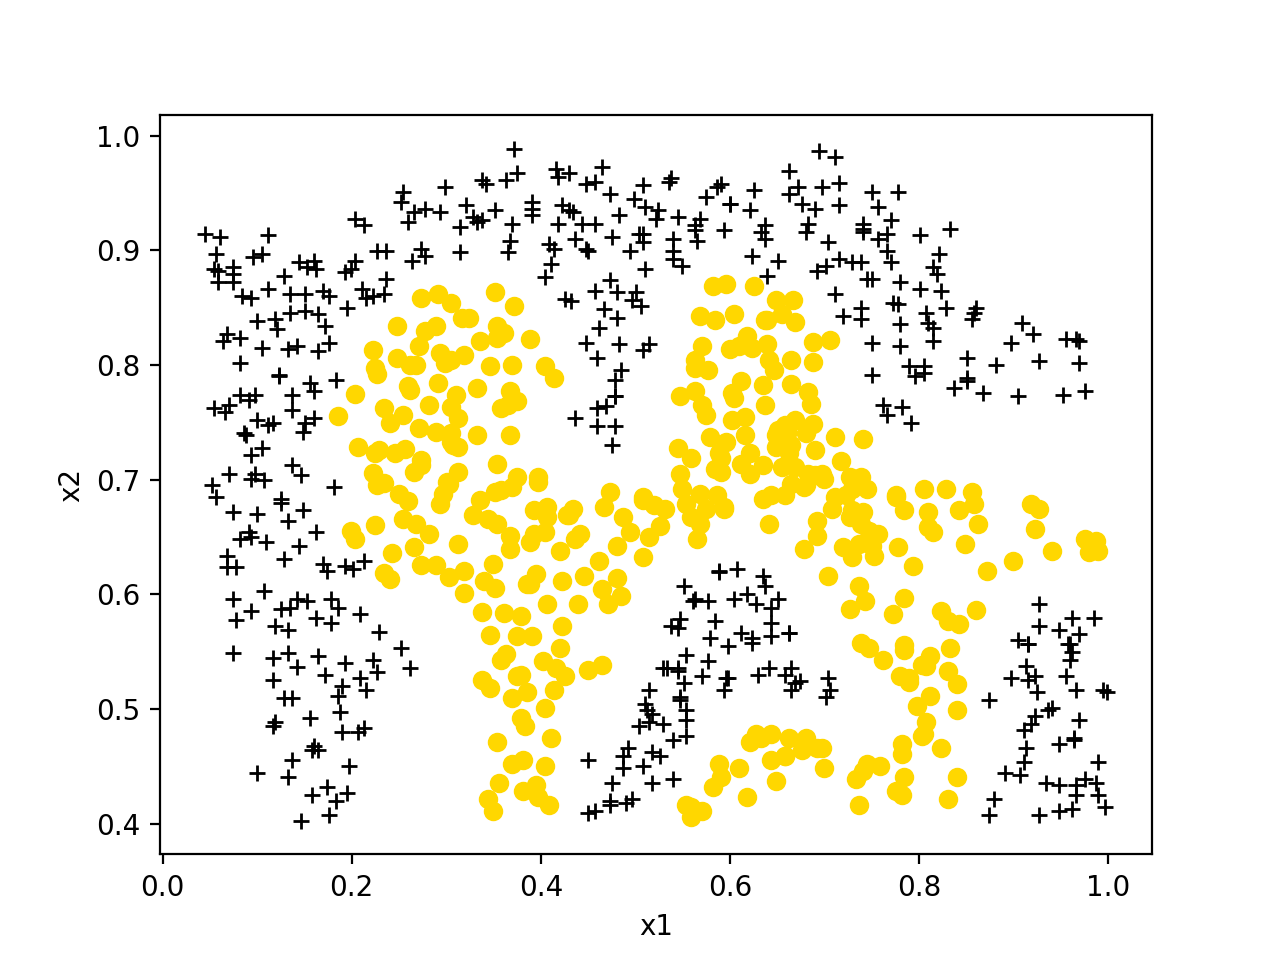
\includegraphics[width=0.4\linewidth]{figs/Chap_10_Figure_2.png}
\end{figure}

\begin{lstlisting}[language=Python]
from sklearn import svm

clf = svm.SVC(C=100, kernel='rbf', gamma=10, probability=True)
clf.fit(X, y)
\end{lstlisting}

训练结果如下：

\begin{figure}[H]
    \centering
    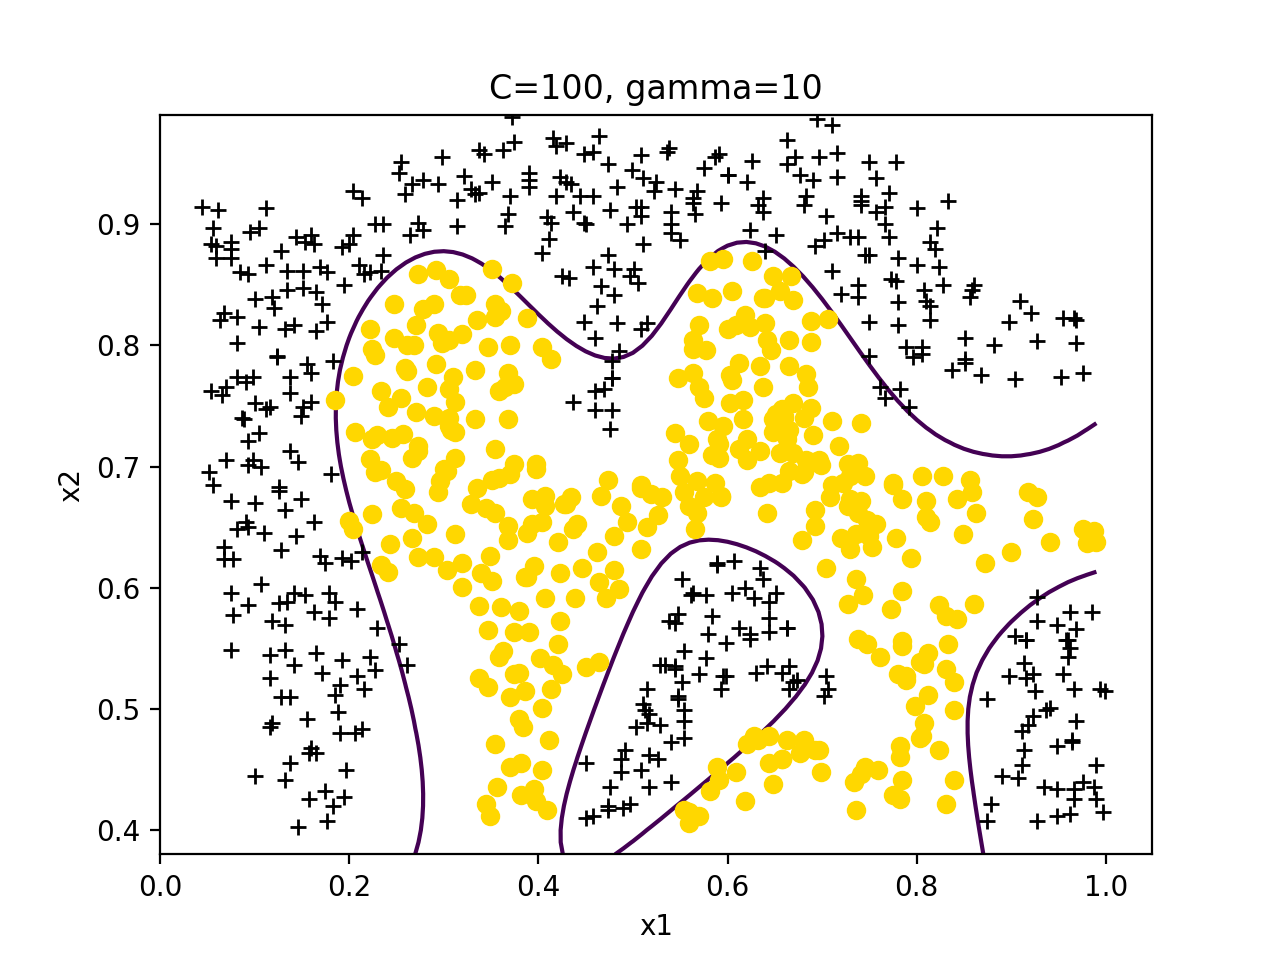
\includegraphics[width=0.4\linewidth]{figs/Chap_10_Figure_2_1.png}
\end{figure}


\paragraph{调整参数 $C,\sigma$}

数据集：

\begin{figure}[H]
    \centering
    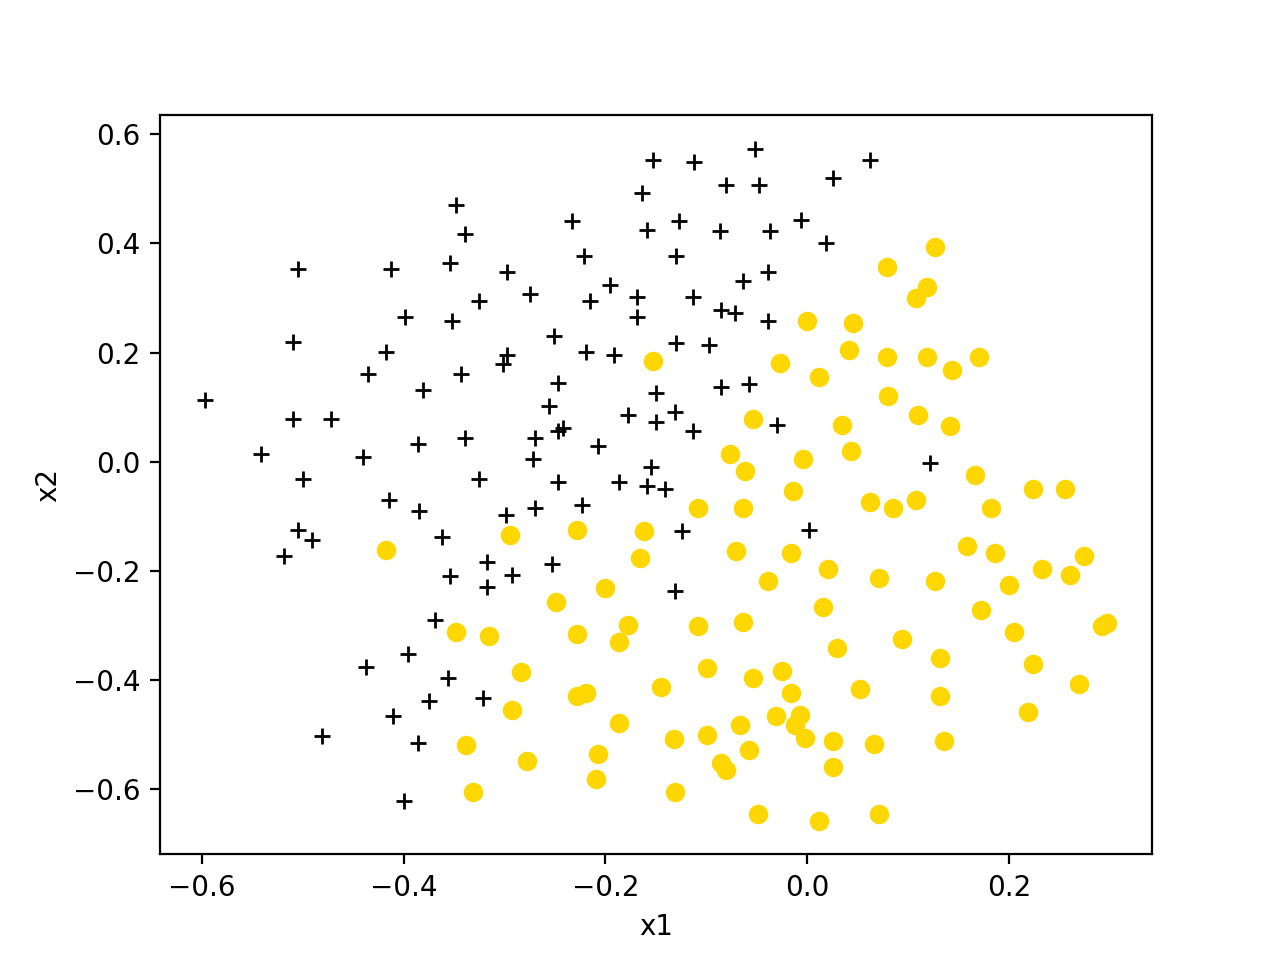
\includegraphics[width=0.4\linewidth]{figs/Chap_10_Figure_3.png}
\end{figure}

\begin{lstlisting}[language=Python]
maxscore, maxC, maxgamma = 0, 0, 0
for C in [0.01, 0.03, 0.1, 0.3, 1, 3, 10, 30]:
	for gamma in [0.01, 0.03, 0.1, 0.3, 1, 3, 10, 30]:
		clf = svm.SVC(C=C, kernel='rbf', gamma=gamma, probability=True)
		clf.fit(X, y)
		score = clf.score(X, y)
		print(C, gamma, score)
		if score > maxscore:
			maxscore, maxC, maxgamma = score, C, gamma

clf = svm.SVC(C=maxC, kernel='rbf', gamma=maxgamma, probability=True)
clf.fit(X, y)
\end{lstlisting}

训练结果如下：

\begin{figure}[H]
    \centering
    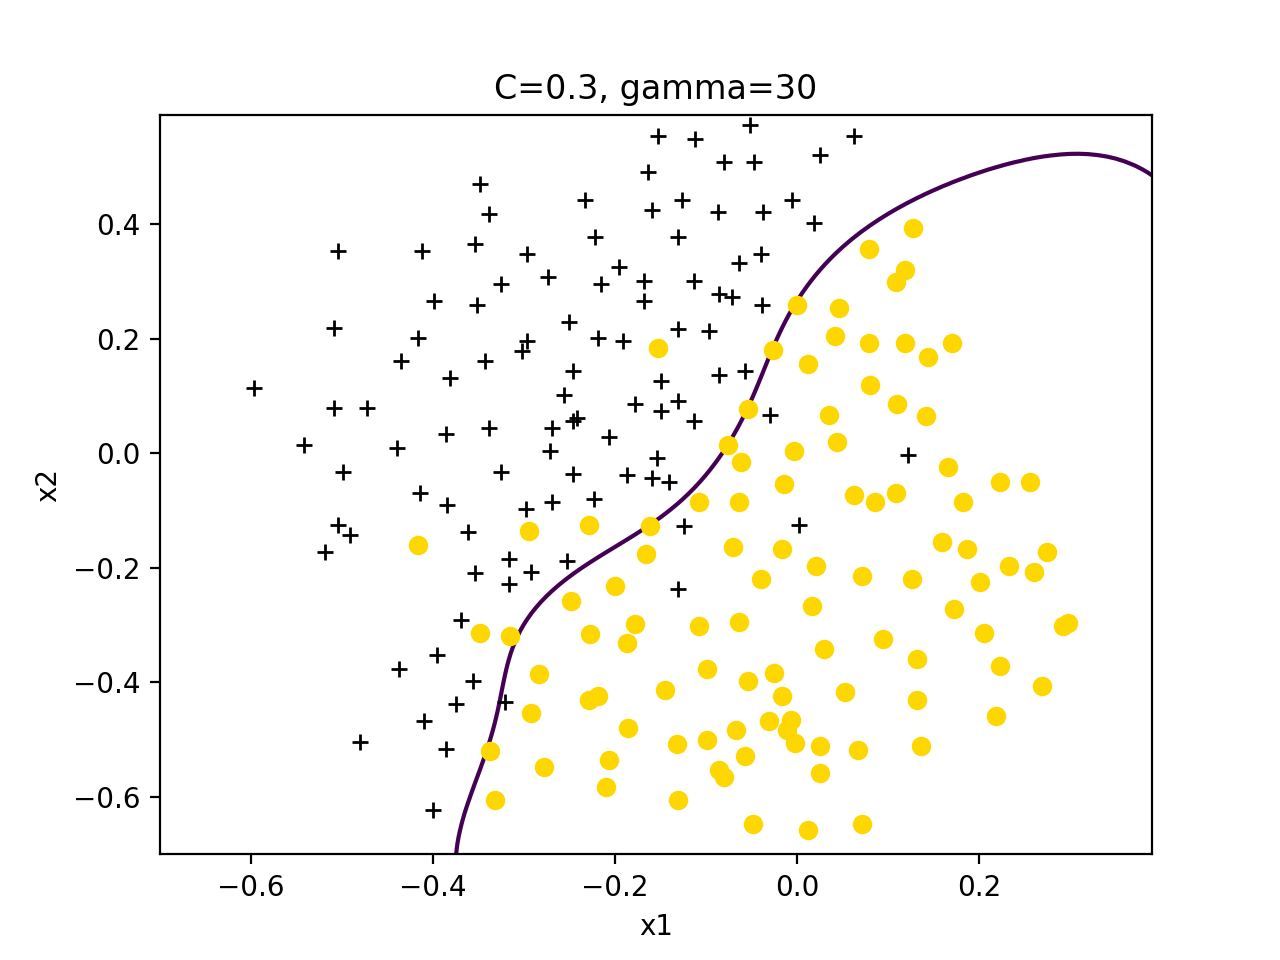
\includegraphics[width=0.4\linewidth]{figs/Chap_10_Figure_3_1.png}
\end{figure}
